%%%%%%%%%%%%%%%%%%%%%%%%%%%%%%%%%%%%%%%%%%%%%%%%%%%%%%%%%%%
% Capitolo 1

\chapter{Contesto ed obiettivi}
\label{ref:contesto}
In questo capitolo sarà introdotto il contesto in cui ci si trova ad operare e gli obiettivi del progetto.


\section{DATABENC}
Il progetto DATABENC (\url{http://www.databenc.it}) (Distretto Ad Alta Tecnologia per i BENi Culturali) è nato in Campania, grazie all'Università degli Studi di Napoli Federico II e all'Università di Salerno, con l'intento di stabilire una programmazione strategica per valorizzare i beni culturali, il patrimonio ambientale e il turismo.
DATABENC ha l'obiettivo di costituire, tra università, centri di ricerca, imprese e amministrazioni comunali presenti sul territorio, una rete che focalizzi le proprie risorse su di un programma di alta tecnologia al fine di creare nuove realtà imprenditoriali (spin-off, start-up), nuove figure professionali, percorsi di alta formazione qualificati, valorizzazione delle conoscenze (brevetti, know how). 
Il distretto è un contenitore in cui riunire ed integrare itinerari eterogenei di ricerca, formazione ed innovazione, con l'obiettivo comune della tutela e della valorizzazione del patrimonio culturale campano inteso in senso esteso: territori, siti, beni e attività. 
\subsection{Le linee di intervento}
Gli ambiti di intervento del Distretto si sviluppano su tre linee portanti: 
\begin{itemize}
\item Conoscenza integrata: la prima forma di tutela di un bene è nella conoscenza e, per tale motivo, è necessario realizzare un esauriente sistema di salvaguardia cognitiva del patrimonio culturale;
\item Monitoraggio diagnostico: ai fini della tutela di un bene risulta indispensabile il monitoraggio diagnostico inteso in senso ampio, che non si limiti solo alla verifica dell'integrità materiale del bene stesso ma si estenda anche all'area in cui il bene è inserito o alle dinamiche turistiche che lo coinvolgono;
\item Fruizione sostenibile: un aspetto fondamentale del bene culturale è quello del suo utilizzo.  Perciò risulta indispensabile conseguire un utilizzo sostenibile del patrimonio culturale.
\end{itemize}

In sintesi, DATABENC ha come obiettivo l'introduzione di una nuova ottica con cui affrontare il grave problema della tutela e della valorizzazione del patrimonio culturale, e la creazione di un sistema che faccia della Campania una regione dell'innovazione e un centro di produzione e diffusione di cultura capace di attrarre capitali economici e, soprattutto, capitali umani.


\section{Ancitel}

Ancitel S.p.A. (\url{http://www.ancitel.it}) è la principale società dell'ANCI - Associazione Nazionale Comuni Italiani - e da 25 anni supporta gli enti locali nella gestione di tutti i processi di innovazione.
Dalla sua fondazione, avvenuta nel 1987,  Ancitel affianca le pubbliche amministrazioni locali con un'ampia rete di servizi e progetti ideati per rispondere alle loro esigenze operative quotidiane.
In quanto partner dei Comuni, Ancitel agisce ed opera ogni giorno come centro di competenza per fornire loro soluzioni e strumenti pensati per facilitarne e supportarne l'azione quotidiana ed affrontare le sfide dell'innovazione. 
Grazie ad una profonda conoscenza delle dinamiche interne alla Pubblica Amministrazione, Ancitel ha conseguito notevoli capacità di ascolto, dialogo ed intervento. Per questo uno dei ruoli fondamentali dell'azienda è quello di promuovere e favorire lo scambio delle informazioni tra gli enti pubblici, centrali e locali.
Grazie alle forti competenze e professionalità e alla capacità di valorizzare le esperienze locali e coinvolgere trasversalmente l'intera rete dei Comuni Italiani, Ancitel è stata scelta come partner affidabile dai principali organismi istituzionali italiani, quali Camera dei Deputati, Presidenza del Consiglio dei Ministri, Ministero dell'Ambiente, Ministero dell'Interno, Ministero del Lavoro e delle Politiche Sociali, Ministero dello Sviluppo Economico, Autorità per l'energia elettrica e il gas.
All'interno del distretto Databenc, Ancitel è uno dei principali soci. 


\section{Fruizione informazioni culturali e turistiche in mobilità}
Nell'ambito dei beni culturali, vi sono diversi progetti che coinvolgono enti locali, grandi, piccole e medie imprese ed istituti universitari.
L'obiettivo comune è quello di sviluppare strumenti di valorizzazione e capitalizzazione dell'offerta culturale e delle risorse ambientali, al fine di promuovere e commercializzare l'offerta turistica da parte delle P.A. locali.
Si rende, quindi, necessaria la definizione e lo sviluppo di una piattaforma abilitante su cui basare servizi per l'offerta culturale. Una piattaforma che ponga al centro le informazioni da offrire agli utenti, che renda facile ed accessibile la fruizione di esse e che possieda validi strumenti per la conservazione e la salvaguardia dei beni culturali.
Le stesse informazioni, inoltre, vanno validate e standardizzate, in modo da consentire facilmente l'estrazione e la catalogazione automatica, l'analisi e la correlazione di esse attraverso motori semantici.
Tra i progetti già in corso, si può citare il campano
\emph{OR.C.HE.S.T.R.A.} (ORganization of Cultural HEritage and Smart Tourism and Real-time Accessibility), il cui partner universitario è l'Università Federico II di Napoli, che ha come obiettivo quello di realizzare un insieme di soluzioni tecnologiche orientate alla valorizzazione del patrimonio culturale, materiale e immateriale, del centro storico di Napoli in ottica Smart. 
%E' altresì auspicabile l'introduzione di un sistema di feedback del bene culturale, in cui è realizzabile il concetto di esplorazione personalizzata in base ad un'analisi delle esperienze degli utenti sul territorio, per comprendere meglio le aspettative del turista influenzato dalle informazioni condivise attraverso i social media.

\section{Gli scavi di Paestum}
Paestum, cittadina della provincia di Salerno, presenta un'area archeologica molto vasta, riconosciuta dall'UNESCO come patrimonio dell'umanità dal 1988.
All'interno di quest'area sono presenti 3 importanti templi, oltre ad altre interessanti testimonianze storico-artistiche. Il \emph{Tempio di Hera} (anche noto come \emph{Basilica} a causa della quasi totale sparizione dei muri della cella, del frontone e della trabeazione) fu dedicato ad Hera, moglie di Zeus, risulta essere il più antico dei 3 templi, essendo stato eretto intorno al 550 a.C.. 
\begin{figure}[h!]
\begin{center}
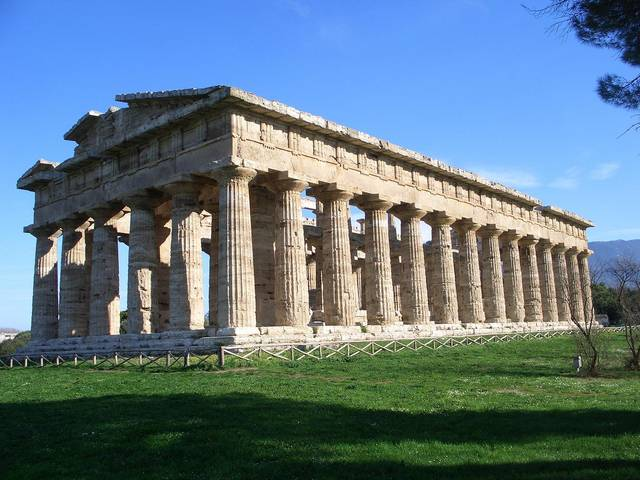
\includegraphics[scale=0.7]{imgs/tempioposeidone.jpg} 
\caption{Tempio di Poseidone\label{tempioposeidone}}
\end{center}
\end{figure}
Il secondo tempio è il \emph{Tempio di Poseidone} (fig. \ref{tempioposeidone}) e incarna il più riuscito esempio di architettura greca in Occidente. Costruito intorno al 450 a.C. seguendo lo stile architettonico dorico classico (lo stesso del Partenone di Atene) risulta orientato da ovest ad est. Il terzo ed ultimo grande tempio è il \emph{Tempio di Cerere}, costruito verso la fine del VI sec. a.C. nel punto più alto della città. Altri punti d'interesse minore sono il \emph{Templio Italico} (dedicato a Giove, Giunone e Minerva, era posto su un alto basamento al cui centro si ergeva un imponente altare e vi si poteva accedere solo dal lato a Sud tramite un'ampia gradinata), il \emph{Foro} (edificato dai romani sulla vecchia Agorà Greca), il \emph{Boleuterion} (detto anche Teatro Greco, fu costruito originariamente per ospitare le riunioni del massimo Consiglio della città ed aveva forma circolare prima di essere ridotto nelle dimensioni dai romani prima sul lato occidentale e poi sul lato settentrionale), l'\emph{Anfiteatro}(destinato agli spettacoli dei Gladiatori e risalente al primo secolo D.C.), il \emph{Ginnasio} (dotato di piscina per gare di nuoto) e il \emph{Sacello Ipogeico} (costruzione sotterranea rinvenuta nel 1954 di cui è ignota la finalità, si suppone che si tratti un tempio sotterraneo dedicato alla dea della fecondità e fertilità, oppure un cenotafio -una tomba simbolica- realizzata per onorare il fondatore della città).
\section{Obiettivi}
Lo scopo di questa tesi è quello di sviluppare, nel contesto di DATABENC, un'applicazione mobile che assista i turisti nella visita del sito archeologico degli scavi di Paestum.
Il turista potrà, sul suo dispositivo mobile, avere a disposizione una mappa su cui poter visualizzare la propria posizione e quella dei punti di interesse presenti nel sito.
Il turista potrà, inoltre, ottenere informazioni approfondite e materiale multimediale su tali punti di interesse. 





\clearpage{\pagestyle{empty}\cleardoublepage}

